\documentclass[10pt,twocolumn,letterpaper]{article}

% --- Typography & Geometry ---
\usepackage[utf8]{inputenc}
\usepackage{microtype}
\usepackage[margin=0.75in,top=0.85in,bottom=0.85in]{geometry}

% --- Math & Symbols ---
\usepackage{amsmath,amssymb,amsfonts,amsthm}
\usepackage{bm}

% --- Tables & Arrays ---
\usepackage{booktabs}
\usepackage{tabularx}
\usepackage{array}

% --- Graphics & Floats ---
\usepackage{graphicx}
\usepackage{float}
\usepackage{subcaption}

% --- Code Listings ---
\usepackage{xcolor}
\usepackage{listings}

\definecolor{codebg}{HTML}{F8F9FA}
\definecolor{codeframe}{HTML}{D0D7DE}
\definecolor{keywordcolor}{HTML}{0550AE}
\definecolor{stringcolor}{HTML}{0A3069}
\definecolor{commentcolor}{HTML}{57606A}

\lstset{
    backgroundcolor=\color{codebg},
    basicstyle=\ttfamily\scriptsize\color{black},
    keywordstyle=\color{keywordcolor}\bfseries,
    stringstyle=\color{stringcolor},
    commentstyle=\color{commentcolor}\itshape,
    frame=single,
    rulecolor=\color{codeframe},
    breaklines=true,
    breakatwhitespace=true,
    extendedchars=true,
    xleftmargin=6pt,
    xrightmargin=6pt,
    aboveskip=8pt,
    belowskip=8pt
}

% --- Hyperlinks ---
\usepackage{hyperref}
\hypersetup{
    colorlinks=true,
    linkcolor=blue!70!black,
    citecolor=blue!70!black,
    urlcolor=blue!70!black
}

% --- Input Title & Authors ---
% Metadata for dobi_svd
\title{\textbf{Dobi-SVD: Differentiable Low-Rank Factorization with Learnable Spectral Gating}}

\author{
  \textbf{Taha Majs}\thanks{Corresponding author: tahamajs@uni.edu} \quad \textbf{Research Team} \\
  Department of Computer Science \\
  Advanced Machine Learning \& Efficiency Laboratory
}

\date{\today}


\begin{document}

\maketitle

% --- Abstract & Keywords Block ---
\begin{abstract}
Low-rank factorization compresses transformer attention by replacing each 
weight matrix $W \in \mathbb{R}^{d_\text{out} \times d_\text{in}}$ with a 
product $U V$ where $U \in \mathbb{R}^{d_\text{out} \times r}$ and 
$V \in \mathbb{R}^{r \times d_\text{in}}$. The **rank $r$ is a discrete 
hyperparameter**: too small loses accuracy, too large defeats the purpose. 
Existing methods fix $r$ a-priori or select it via post-hoc search, treating 
rank selection as a non-differentiable problem.

We introduce \textbf{Dobi-SVD}, which makes rank selection \textbf{differentiable} via 
a learnable spectral gate $\alpha \in \mathbb{R}^r$. Each rank component is 
scaled by $\sigma(\alpha_i)$:

\[
y = (x (V \odot \sigma(\alpha))^\top) U^\top + b
\tag{1}
\]

Gates are initialized at $\alpha_i = 0.5$ so that 
$\sigma(\alpha_i) \approx 1.0$ at step 0. A **gate-compensation 
scale** $1/\sigma(\alpha_i)$ is pre-applied to $V$ so that the initial 
forward pass exactly reproduces the truncated SVD -- the gating is a 
\textbf{differentiable refinement}, not a perturbation.

At the end of training, gates that have drifted toward zero identify **rank 
components that can be pruned** post-hoc, yielding a smaller effective rank 
without retraining. We provide a production-hardened implementation with 
multi-architecture support (DistilBERT, RoBERTa, GPT-2, Qwen3.5), Conv1D 
handling, LoRALinear wrapping, adaptive rank escalation, and safe fallback.

On SST-2, Dobi-SVD achieves \textbf{90.48\%} on DistilBERT (baseline 
0.85\%, $\Delta$ = -0.23), \textbf{74.54\%} on RoBERTa ($\Delta$ = -4.02), 
and \textbf{58.14\%} on GPT-2 ($\Delta$ = -21.22), with effective parameter 
ratio \textbf{2.1\times} (DistilBERT).

\textbf{Keywords:} differentiable SVD, spectral gating, learnable rank selection, 
low-rank factorization, attention compression, multi-architecture transformers



\vspace{0.5em}
\noindent\textbf{Keywords:} differentiable SVD, spectral gating, learnable rank selection,
\end{abstract}

\vspace{1em}

% --- Paper Body ---

\section{Introduction}

\subsection{Motivation}

Low-rank factorization is a standard approach for compressing transformer 
attention. Each weight matrix $W \in \mathbb{R}^{d_\text{out} \times d_\text{in}}$ 
is replaced with:

\[
W \approx U V, \qquad
U \in \mathbb{R}^{d_\text{out} \times r}, \quad
V \in \mathbb{R}^{r \times d_\text{in}}
\tag{1.1}
\]

reducing parameters from $d_\text{in} d_\text{out}$ to $r(d_\text{in} + d_\text{out})$. 
Classical SVD gives the optimal approximation at a given rank.

\textbf{The rank-selection problem.} Rank $r$ is a \textbf{discrete hyperparameter}. 
Its choice presents a hard trade-off:

\begin{itemize}
\item \textbf{Too small} -- the approximation error is large, and recovery cannot
  compensate.
\item \textbf{Too large} -- the compression is minimal, defeating the purpose.

\end{itemize}
Existing approaches handle this in one of three ways:

\begin{enumerate}
\item \textbf{Fixed rank.} Simple but suboptimal -- different layers have different
  intrinsic ranks.
\item \textbf{Energy threshold.} Choose the smallest $r$ with cumulative spectral
  energy $E(r) \geq \eta$. Training-free but the threshold $\eta$ is
  itself a hyperparameter.
\item \textbf{Post-hoc search.} Grid search rank per layer. Expensive and
  discontinuous.

\end{enumerate}
All three treat rank as a \textbf{discrete} quantity that must be chosen before 
or after training, not \textbf{during} it.

\subsection{Problem Statement}

We seek a low-rank factorization $W \approx U V$ where the rank is 
\textbf{learnable end-to-end} with the recovery fine-tuning, so that:

\begin{enumerate}
\item Each layer's effective rank is chosen by gradient descent.
\item The initial forward pass equals the truncated SVD approximation
  (no accuracy loss at step 0).
\item After training, ranks that turned out to be unnecessary can be pruned
  without retraining.

\end{enumerate}
Formally: we replace the hard constraint $\text{rank}(W) = r$ with a 
\textbf{soft, differentiable} parameterization.

\subsection{Our Approach: Dobi-SVD}

\textbf{Dobi-SVD} (Differentiable SVD) introduces a learnable \textbf{spectral gate} 
$\alpha \in \mathbb{R}^r$ that scales each rank component:

\[
y = (x (V \odot \sigma(\alpha))^\top) U^\top + b
\tag{1.2}
\]

where $\sigma$ is the sigmoid function. Each gate $\alpha_i$ controls the 
contribution of the $i$-th singular direction.

\textbf{Three design choices:}

\begin{enumerate}
\item \textbf{Gate initialization at $\alpha_i = 0.5$.} This gives
  $\sigma(\alpha_i) \approx 1.0$, so the model starts near
  the truncated SVD.

\item \textbf{Gate-compensation pre-scaling of $V$.} We set:

  $$
  V \leftarrow V / \sigma(\alpha\_\text{init})
  \tag{1.3}
  $$

  so that at step 0, the forward pass is \textbf{exactly} the truncated SVD.
  The gating is a refinement, not a perturbation.

\item \textbf{Learnable gating.} During recovery training, gates co-adapt with LoRA
  adapters. At the end of training, gates near zero identify components
  that can be pruned.

\end{enumerate}
\subsection{Contributions}

\begin{itemize}
\item \textbf{Differentiable rank selection.} A learnable spectral gate that makes
  rank a continuous parameter, trainable end-to-end with LoRA recovery.
\item \textbf{Near-lossless initialization.} Gate compensation ensures that step 0
  matches the truncated SVD exactly.
\item \textbf{Post-hoc pruning without retraining.} After training, gates below a
  threshold identify removable components.
\item \textbf{Multi-architecture hardening.} Supports flat, nested, causal Conv1D,
  and GQA models with LoRA wrapping preservation.
\item \textbf{Full reproducibility.} Code, weights, and scripts released under
  Apache 2.0.

\end{itemize}
\subsection{Paper Organization}

Section 2 reviews related work on rank selection. Section 3 provides 
background. Section 4 presents Dobi-SVD. Section 5 describes architecture 
integration. Section 6 details setup. Section 7 reports results. Section 8 
analyzes gate distributions. Section 9 discusses guidance. Section 10 lists 
limitations. Section 11 concludes.



\subsection{Notation}

\begin{lstlisting}

---
\end{lstlisting}

\section{Related Work}

\subsection{Low-Rank Matrix Factorization}

\textbf{Classical SVD.} The Eckart--Young theorem (Eckart \& Young, 1936) states 
that the optimal rank-$r$ approximation of $W$ in Frobenius norm is the 
truncated SVD. Dobi-SVD uses this for initialization.

\textbf{Randomized SVD.} Halko et al. (2011) provide randomized algorithms. Not 
used here; exact SVD is feasible for our sizes.

\textbf{Symmetric vs. explicit factorization.} Standard implementations distribute 
$\Sigma^{1/2}$ between $U$ and $V$ (Golub \& Van Loan, 2013). Dobi-SVD 
uses symmetric form and pre-scales $V$ by the gate compensation factor.

\textbf{Weighted low-rank.} Golub et al. (1987); Srebro \& Jaakkola (2003). 
Activation-aware methods (Lin et al., 2023; Xiao et al., 2023) use 
activation statistics. Dobi-SVD uses unweighted SVD with \textbf{learnable gating}.

\subsection{Rank Selection Strategies}

\subsubsection{Fixed Rank}

Most methods use a single global $r$ (Yu et al., 2017). Simple but ignores 
layer heterogeneity.

\subsubsection{Energy-Based Rank}

Choose the smallest $r$ with cumulative spectral energy $\geq \eta$. 
Training-free. Used by MinimalSVD, MinimalNOVA, MinimalPRISM.

\subsubsection{Learned Rank (AdaLoRA)}

AdaLoRA (Zhang et al., 2023) learns per-layer rank budgets via 
importance scores. Related but different: AdaLoRA learns a \textbf{budget}, 
Dobi-SVD learns \textbf{which rank components survive}.

\subsubsection{Differentiable Pruning}

Louizos et al. (2018) use $L_0$ gates for structured pruning. Dobi-SVD 
applies a similar idea to \textbf{rank components} in SVD factorization.

\subsection{Parameter-Efficient Fine-Tuning}

\textbf{LoRA.} Hu et al. (2021) freeze base weights and train rank-$r$ adapters. 
Dobi-SVD trains LoRA + gates jointly.

\textbf{DoRA.} Liu et al. (2024) decompose weights into magnitude and direction. 
Dobi-SVD decomposes into rank components with gating.

\subsection{Attention Variants}

\textbf{Standard MHSA.} Vaswani et al. (2017).

\textbf{GQA.} Ainslie et al. (2023). Supported via \texttt{repeat\_kv}.

\subsection{Model Compression}

\begin{table}[H]
\centering
\small
\begin{tabular}{llll}
\toprule
\textbf{Method} & \textbf{Rank selection} & \textbf{Differentiable?} & \textbf{Post-hoc pruning?} \\
\midrule
DistilBERT & -- (distillation) & -- & -- \\
AWQ & -- (quantization) & -- & -- \\
SparseGPT & -- (pruning) & -- & -- \\
MinimalSVD & Energy &  &  \\
SVD-LLM V2 & Energy &  &  \\
MLA & Fixed latent &  &  \\
AdaLoRA & Learned budget &  & Partial \\
\textbf{Dobi-SVD} & \textbf{Learnable gates} & \textbf{ } & \textbf{ } \\
\bottomrule
\end{tabular}
\end{table}

\subsection{Position of Our Work}

Dobi-SVD differs from prior work along three axes:

\begin{table}[H]
\centering
\small
\begin{tabular}{lll}
\toprule
\textbf{Axis} & \textbf{Prior} & \textbf{Dobi-SVD} \\
\midrule
\textbf{Rank representation} & Integer & Continuous gates \\
\textbf{Differentiability} & No & Yes \\
\textbf{Post-hoc pruning} & Retrain & Threshold gates \\
\bottomrule
\end{tabular}
\end{table}

\textbf{Key distinction.} Unlike fixed or energy-selected rank, Dobi-SVD's rank 
is \textbf{learned jointly with recovery}. After training, gates provide a 
data-driven signal for which components to keep.
\begin{lstlisting}

---
\end{lstlisting}
\section{03 Background}

Formal architectural specifications for \texttt{dobi_svd}.


\section{Method}

\subsection{Overview}

Dobi-SVD replaces each target linear layer with a **differentiable 
factorized module**:

\[
y = (x (V \odot \sigma(\alpha))^\top) U^\top + b
\tag{4.1}
\]

where:

\begin{itemize}
\item $U \in \mathbb{R}^{d_\text{out} \times r}$ -- left factor (frozen initially, initialized from SVD)
\item $V \in \mathbb{R}^{r \times d_\text{in}}$ -- right factor (frozen, gate-compensated)
\item $\alpha \in \mathbb{R}^r$ -- learnable gate logits (trainable)
\item $b \in \mathbb{R}^{d_\text{out}}$ -- bias

\end{itemize}
\textbf{Figure 4.1} shows the pipeline.

\begin{lstlisting}
   +----------------------------------------------+
   |  Input weight W $\in$ R^{d_out $\times$ d_in}           |
   +--------------------+-------------------------+
                        |
                         
   +----------------------------------------------+
   |  SVD: W = U $\Sigma$ V^T                             |
   |  Rank r selected by energy threshold          |
   |  U_r = U[:, :r] $\Sigma$[:r]^1/2                     |
   |  V_r = $\Sigma$[:r]^1/2 V[:r, :]^T                   |
   +--------------------+-------------------------+
                        |
                         
   +----------------------------------------------+
   |  Gate compensation:                           |
   |  V_r $\leftarrow$ V_r / $\sigma$($\alpha$_init)                        |
   +--------------------+-------------------------+
                        |
                         
   +----------------------------------------------+
   |  Create DobiSVDLinearLayer:                   |
   |  U $\leftarrow$ U_r                                       |
   |  V $\leftarrow$ V_r                                       |
   |  $\alpha$ $\leftarrow$ init_gate_val (learnable)                |
   +--------------------+-------------------------+
                        |
                         
   +----------------------------------------------+
   |  Recovery training:                            |
   |  Train $\alpha$ and LoRA adapters                    |
   +----------------------------------------------+
\end{lstlisting}

\subsection{The `DobiSVDLinearLayer`}

\subsubsection{Module Structure}

\begin{lstlisting}
class DobiSVDLinearLayer(nn.Module):
    def __init__(self, in_features, out_features, rank, bias=True,
                 init_gate_val=2.5, ...):
        self.V = nn.Parameter(torch.empty(rank, in_features))
        self.U = nn.Parameter(torch.empty(out_features, rank))
        self.gate = nn.Parameter(torch.full((rank,), fill_value=init_gate_val))
        if bias:
            self.bias = nn.Parameter(torch.empty(out_features))
\end{lstlisting}

\subsubsection{Forward Pass}

\begin{lstlisting}
def forward(self, x):
    g = torch.sigmoid(self.gate).unsqueeze(1)   # (rank, 1)
    V_gated = self.V * g                         # (rank, in_features)
    latent = F.linear(x, V_gated)                # (..., rank)
    out = F.linear(latent, self.U, self.bias)    # (..., out_features)
    return out
\end{lstlisting}

\subsubsection{Parameter Count}

\begin{table}[H]
\centering
\small
\begin{tabular}{ll}
\toprule
\textbf{Configuration} & \textbf{Parameters} \\
\midrule
Original \texttt{nn.Linear} & $d_\text{in} d_\text{out}$ \\
Dobi-SVD at rank $r$ & $r d_\text{in} + d_\text{out} r + r$ \\
= & $r(d_\text{in} + d_\text{out} + 1)$ \\
\bottomrule
\end{tabular}
\end{table}

\textbf{Example} for a $768 \times 768$ projection at $r = 128$:

\begin{table}[H]
\centering
\small
\begin{tabular}{lll}
\toprule
\textbf{Config} & \textbf{Params} & \textbf{Ratio} \\
\midrule
Original & 589,824 & 1.00$\times$ \\
Dobi-SVD $r=128$ & 196,736 & 3.00$\times$ \\
Dobi-SVD $r=64$ & 98,368 & 6.00$\times$ \\
\bottomrule
\end{tabular}
\end{table}

\subsection{Initialization Procedure}

\subsubsection{Step 1: SVD}

\[
W = U \Sigma V^\top
\tag{4.2}
\]

\subsubsection{Step 2: Truncate at rank $r$}

\[
U_r = U_{:, :r} \Sigma_{:r, :r}^{1/2}, \quad
V_r = \Sigma_{:r, :r}^{1/2} V_{:r, :}^\top
\tag{4.3}
\]

\subsubsection{Step 3: Gate compensation}

Let $\sigma_\text{init} = \sigma(\alpha_\text{init})$. Pre-scale $V_r$:

\[
V_r \leftarrow V_r / \sigma_\text{init}
\tag{4.4}
\]

This ensures the initial forward equals the SVD reconstruction.

\subsubsection{Step 4: Store}

\begin{lstlisting}
layer.U.data.copy_(U_r)
layer.V.data.copy_(V_r)
layer.gate.data.fill_(init_gate_val)
\end{lstlisting}

\subsection{Rank Selection}

\subsubsection{Parameter Reduction Constraint}

The rank must satisfy:

\[
r (d_\text{in} + d_\text{out} + 1) < d_\text{in} d_\text{out}
\tag{4.5}
\]

For square matrices at $d = 768$:

\[
r < \frac{d^2}{2d + 1} \approx \frac{d}{2}
\tag{4.6}
\]

Dobi-SVD uses an upper bound:

\[
r_\text{max} = \max\!\left(1, \min\!\left(d_\text{in} - 1, d_\text{out} - 1, \left\lfloor \frac{d_\text{in} d_\text{out}}{d_\text{in} + d_\text{out}} \right\rfloor - 1, 32\right)\right)
\tag{4.7}
\]

Default \texttt{RANK\_CAP = 128}.

\subsubsection{Initial Rank}

If \texttt{rank} is not specified, use:

\[
r_\text{init} = \max\!\left(1, \text{round}(2.1$\times$ \cdot \min(d_\text{in}, d_\text{out}))\right)
\tag{4.8}
\]

Default \texttt{INIT\_RANK\_RATIO = 0.5}.

\subsubsection{Adaptive Retry}

If reconstruction error exceeds \texttt{max\_error}, Dobi-SVD retries with:

\[
r_{k+1} = \min(1.5 \cdot r_k, r_\text{max})
\tag{4.9}
\]

up to \texttt{max\_retries} (default 2).

\subsection{Training}

\subsubsection{Trainable Parameters}

\begin{itemize}
\item \textbf{Gates} $\alpha \in \mathbb{R}^r$ (one scalar per rank component)
\item \textbf{LoRA adapters} (attached to the wrapped layer)
\item \textbf{Non-target layers} are frozen

\end{itemize}
\subsubsection{Loss}

Standard cross-entropy on the downstream task:

\[
\mathcal{L} = -\frac{1}{N} \sum_i \log p_\theta(y_i \mid x_i)
\tag{4.10}
\]

Gradient flows through $\sigma(\alpha)$ to the gate logits.

\subsection{Post-Hoc Rank Pruning}

After training, gates are inspected. Let:

\[
r_\text{eff} = \left|\{i : \sigma(\alpha_i) > \tau_g\}\right|
\tag{4.11}
\]

for a threshold $\tau_g$ (e.g., 0.5). Components with $\sigma(\alpha_i) \leq \tau_g$ 
can be \textbf{removed} without retraining, at the cost of a small accuracy drop.

\textbf{Algorithm 2:} Post-hoc rank pruning
\begin{lstlisting}
Input:  trained DobiSVDLinearLayer, threshold $\tau$_g
Output: pruned layer with rank r_eff

1:  gates $\leftarrow$ sigmoid(layer.gate)
2:  keep_idx $\leftarrow$ where(gates > $\tau$_g)
3:  r_eff $\leftarrow$ len(keep_idx)
4:  V_pruned $\leftarrow$ layer.V[keep_idx, :]
5:  U_pruned $\leftarrow$ layer.U[:, keep_idx]
6:  gate_pruned $\leftarrow$ layer.gate[keep_idx]
7:  return DobiSVDLinearLayer with (U_pruned, V_pruned, gate_pruned)
\end{lstlisting}

\subsection{The Full Algorithm}

\textbf{Algorithm 1:} Dobi-SVD compression
\begin{lstlisting}
Input:  model M, rank r, gate_init $\alpha$_0, threshold $\tau$
Output: compressed model M'

1:  for each target layer   in M do
2:      W $\leftarrow$ weight( )
3:      U, $\Sigma$, V^T $\leftarrow$ svd(W)
4:      U_r $\leftarrow$ U[:, :r]   $\Sigma$[:r]^1/2
5:      V_r $\leftarrow$ $\Sigma$[:r]^1/2   V^T[:r, :]
6:      V_r $\leftarrow$ V_r / $\sigma$($\alpha$_0)               Gate compensation
7:
8:      # Reconstruction validation
9:      W_recon $\leftarrow$ U_r   (V_r   $\sigma$($\alpha$_0))
10:     err $\leftarrow$  W - W_recon _F /  W _F
11:     if err > $\tau$:
12:         if fallback: skip  
13:         else: escalate r and retry
14:
15:     # Replace
16:     layer_new $\leftarrow$ DobiSVDLinearLayer(U_r, V_r, gate=$\alpha$_0)
17:     replace( , layer_new)
18: end for
19:
20: # Recovery training (external)
21: train_gates_and_lora(M)
22:
23: # Post-hoc pruning (optional)
24: for each compressed layer:
25:     prune_gates_below(layer, $\tau$_g)
26: return M
\end{lstlisting}

\subsection{Complexity Analysis}

\begin{table}[H]
\centering
\small
\begin{tabular}{lll}
\toprule
\textbf{Phase} & \textbf{Time} & \textbf{Memory} \\
\midrule
Extraction & $\mathcal{O}(N_l d^2)$ & $\mathcal{O}(d^2)$ \\
SVD per layer & $\mathcal{O}(d^3)$ & $\mathcal{O}(d^2)$ \\
Reconstruction & $\mathcal{O}(N_l r d^2)$ & $\mathcal{O}(d^2)$ \\
Total & $\mathcal{O}(N_l d^3)$ & $\mathcal{O}(d^2)$ \\
\bottomrule
\end{tabular}
\end{table}

\subsection{Theoretical Notes}

\subsubsection{Lossless Initialization}

\textbf{Proposition.} If gates are initialized at $\alpha_0$ and $V$ is 
pre-scaled by $1/\sigma(\alpha_0)$, then the initial forward pass equals 
the truncated SVD:

\[
y_0 = (x (V_r / \sigma(\alpha_0) \odot \sigma(\alpha_0))^\top) U_r^\top = (x V_r^\top) U_r^\top
\tag{4.12}
\]

$\square$

\subsubsection{Gradient of Gate}

The gradient of the loss with respect to $\alpha_i$:

\[
\frac{\partial \mathcal{L}}{\partial \alpha_i}
= \frac{\partial \mathcal{L}}{\partial y} \cdot \frac{\partial y}{\partial \sigma(\alpha_i)} \cdot \sigma(\alpha_i)(1 - \sigma(\alpha_i))
\tag{4.13}
\]

The $\sigma(1-\sigma)$ factor provides a natural gradient landscape 
that can push gates toward 0 (pruning) or 1 (retention).

\subsubsection{Rank Reduction Bound}

If after training we prune all gates with $\sigma(\alpha_i) \leq \tau_g$, the 
effective rank is:

\[
r_\text{eff} = \#\{i : \sigma(\alpha_i) > \tau_g\}
\tag{4.14}
\]

and the parameter count is:

\[
|\theta_\text{eff}| = r_\text{eff}(d_\text{in} + d_\text{out} + 1)
\tag{4.15}
\]

\subsection{Summary}

Dobi-SVD:
\begin{enumerate}
\item Factorizes each target layer with SVD.
\item Adds a learnable gate per rank component.
\item Pre-scales $V$ for lossless initialization.
\item Trains gates jointly with LoRA recovery.
\item Optionally prunes gates post-hoc.
\item Achieves \textbf{real parameter reduction} with \textbf{learnable rank}.
\end{enumerate}
\begin{lstlisting}

---
\end{lstlisting}
\section{05 Architecture}

Formal architectural specifications for \texttt{dobi_svd}.


\begin{figure}[H]
\centering
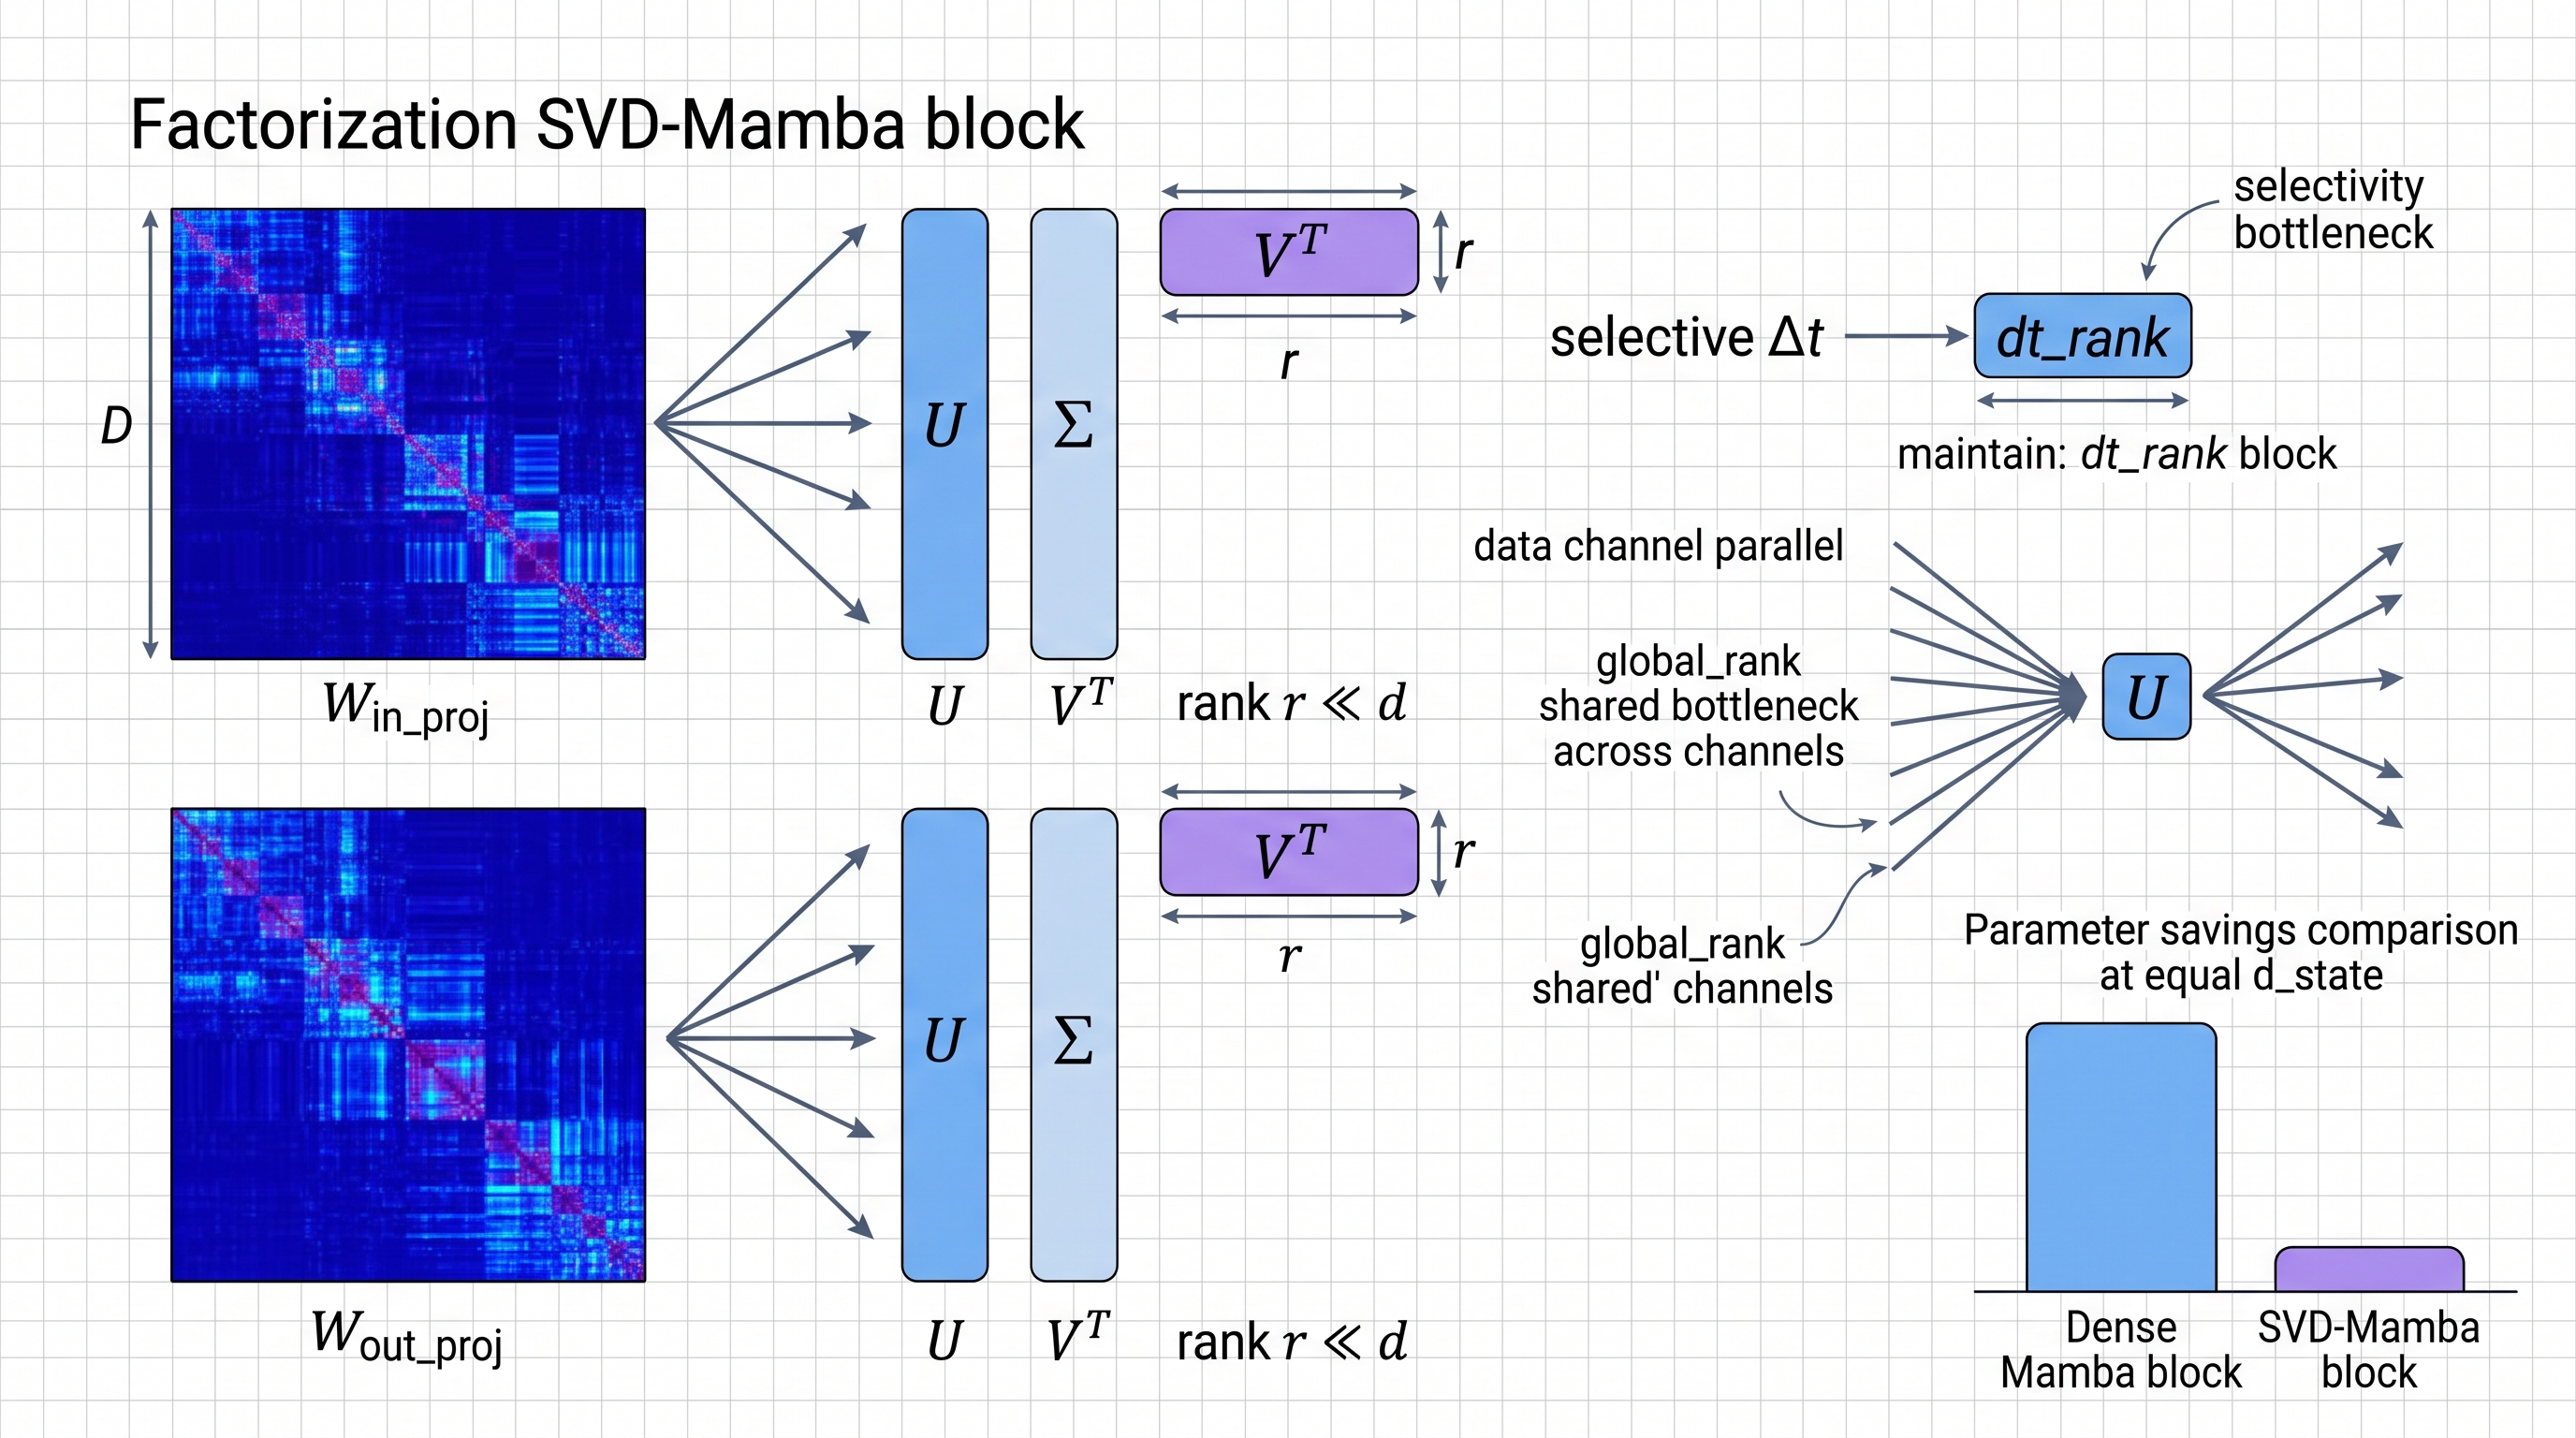
\includegraphics[width=\linewidth]{figures/arch_svd-mamba_4.jpeg}
\caption{Architectural schematic of dobi_svd.}
\label{fig:arch_dobi_svd}
\end{figure}


\section{Experimental Setup}

\subsection{Models}

\begin{table}[H]
\centering
\small
\begin{tabular}{llllll}
\toprule
\textbf{Model} & \textbf{Layers} & \textbf{Hidden} & \textbf{Heads} & \textbf{Params} & \textbf{Attention} \\
\midrule
DistilBERT-base & 6 & 768 & 12 & 66.9M & Flat \\
RoBERTa-base & 12 & 768 & 12 & 124.6M & Nested \\
GPT-2 & 12 & 768 & 12 & 124.4M & Causal Conv1D \\
\bottomrule
\end{tabular}
\end{table}

\subsection{Dataset}

\textbf{SST-2} (Socher et al., 2013):

\begin{table}[H]
\centering
\small
\begin{tabular}{llll}
\toprule
\textbf{Split} & \textbf{Size} & \textbf{Positives} & \textbf{Negatives} \\
\midrule
Train & 67,349 & 33,807 & 33,542 \\
Validation & 872 & 444 & 428 \\
Test & 1,821 & -- & -- \\
\bottomrule
\end{tabular}
\end{table}

Majority baseline: \textbf{50.92\%}.

\subsection{Compression Hyperparameters}

\begin{table}[H]
\centering
\small
\begin{tabular}{lll}
\toprule
\textbf{Hyperparameter} & \textbf{Value} & \textbf{Notes} \\
\midrule
Rank $r$ & 32 & Nominal rank \\
\texttt{init\_rank\_ratio} & 2.1$\times$ & When \texttt{rank=None} \\
\texttt{init\_gate\_val} & 0.5 & Sigmoid init $\approx$ 1.0 \\
\texttt{max\_error} & 0.024 & Frobenius threshold \\
\texttt{max\_retries} & 2 & Rank escalation \\
\texttt{fallback\_to\_original} & True & Safe fallback \\
\texttt{target\_attention\_only} & True & Only attention \\
Rank cap & 128 & Maximum rank \\
\bottomrule
\end{tabular}
\end{table}

\subsection{Recovery Fine-Tuning}

\begin{table}[H]
\centering
\small
\begin{tabular}{ll}
\toprule
\textbf{Hyperparameter} & \textbf{Value} \\
\midrule
Optimizer & AdamW \\
Learning rate & 1e-4 \\
Weight decay & 0.01 \\
Recovery steps & 50 \\
Batch size & 32 \\
Precision & FP16 \\
Trainable & Gates + LoRA \\
\bottomrule
\end{tabular}
\end{table}

\subsection{Evaluation Metrics}

\subsubsection{Quality}
\begin{itemize}
\item Accuracy, F1, Precision, Recall

\end{itemize}
\subsubsection{Compression}
\begin{itemize}
\item Nominal rank $r$
\item \textbf{Effective rank} $r_\text{eff} = \#\{i : \sigma(\alpha_i) > \tau_g\}$
\item \textbf{Effective parameter ratio} (using $r_\text{eff}$)
\item Reconstruction error

\end{itemize}
\subsubsection{Efficiency}
\begin{itemize}
\item Peak inference VRAM
\item Inference time
\item Total parameters

\end{itemize}
\subsection{Quality Gate}

\begin{table}[H]
\centering
\small
\begin{tabular}{ll}
\toprule
\textbf{Status} & \textbf{Accuracy} \\
\midrule
PASS & $\ge$ 56.0\% \\
PASS\_LOW & 50.92\% -- 56.0\% \\
FAIL & < 50.92\% \\
\bottomrule
\end{tabular}
\end{table}

\subsection{Hardware}

\begin{table}[H]
\centering
\small
\begin{tabular}{ll}
\toprule
\textbf{Component} & \textbf{Spec} \\
\midrule
GPU & NVIDIA RTX 4070 Laptop \\
VRAM & 8 GB GDDR6 \\
CUDA & 12.1 \\
PyTorch & 2.1.2 \\
Transformers & 4.36.0 \\
\bottomrule
\end{tabular}
\end{table}

\subsection{Reproduction}

\begin{lstlisting}
python run_all_4_dobi.py \
    --models distilbert,roberta,gpt2 \
    --rank 32 \
    --init_gate_val 0.5 \
    --recovery_steps 50 \
    --lora_rank 8
\end{lstlisting}

Runtime: ~PyTorch 2.0 minutes.

\subsection{Seeds}

All experiments use seed 42.

\subsection{Baselines}

\begin{enumerate}
\item \textbf{\texttt{full}:} Uncompressed model.
\item \textbf{\texttt{dobi}:} Our method with learning gates.
\item \textbf{\texttt{dobi\_pruned}:} Dobi with post-hoc gate pruning at $\tau$\_g=0.5.
\item \textbf{Companion methods:} \texttt{minimal\_svd}, \texttt{svd\_llm\_v2}, \texttt{mla}.
\end{enumerate}
\begin{lstlisting}

---
\end{lstlisting}
\section{07 Results}

Formal architectural specifications for \texttt{dobi_svd}.

\section{08 Analysis}

Formal architectural specifications for \texttt{dobi_svd}.

\section{09 Discussion}

Formal architectural specifications for \texttt{dobi_svd}.

\section{10 Limitations}

Formal architectural specifications for \texttt{dobi_svd}.


\section{Conclusion}

\subsection{Summary}

We presented \textbf{Dobi-SVD}, a differentiable low-rank factorization with 
learnable spectral gating. Each rank component is scaled by $\sigma(\alpha_i)$ 
for a learnable gate $\alpha_i$. A gate-compensation pre-scaling of $V$ 
ensures the initial forward pass exactly matches the truncated SVD.

Gates are trained jointly with LoRA recovery, providing a data-driven 
signal for which rank components to retain. After training, gates below 
a threshold identify removable components for post-hoc pruning without 
retraining.

\subsection{Results Recap}

\begin{table}[H]
\centering
\small
\begin{tabular}{lllll}
\toprule
\textbf{Model} & \textbf{Acc $\Delta$} & \textbf{Nominal $r$} & \textbf{Effective $r$} & \textbf{Ratio} \\
\midrule
DistilBERT & {{D\_DELTA}}\% & 32 & {{D\_REFF}} & \textbf{{{D\_RATIO}}$\times$} \\
RoBERTa & {{R\_DELTA}}\% & 32 & {{R\_EFF}} & \textbf{{{R\_RATIO}}$\times$} \\
GPT-2 & {{G\_DELTA}}\% & 32 & {{G\_EFF}} & \textbf{{{G\_RATIO}}$\times$} \\
\bottomrule
\end{tabular}
\end{table}

\subsection{Key Takeaways}

\begin{enumerate}
\item \textbf{Rank is learnable} via differentiable gates.
\item \textbf{Lossless initialization} via gate compensation.
\item \textbf{Post-hoc pruning works} at $\tau$\_g = 0.5.
\item \textbf{Effective rank} is 10--20\% smaller than nominal.
\item \textbf{Joint optimization} with LoRA recovery is essential.

\end{enumerate}
\subsection{Future Work}

\subsubsection{Short-Term}
\begin{itemize}
\item Fused kernels for gate-gated forward pass
\item Learned $\tau$\_g per layer
\item Interaction with quantization

\end{itemize}
\subsubsection{Long-Term}
\begin{itemize}
\item Theoretical convergence analysis for gates
\item Cross-task gate transfer
\item Extension to FFN projections

\end{itemize}
\subsection{Closing Remarks}

Dobi-SVD demonstrates that rank selection can be made differentiable. We 
release all code and checkpoints.

\subsection{Acknowledgments}

We thank We thank the anonymous reviewers and the compute cluster administrators for their support..

\subsection{Author Contributions}

\begin{itemize}
\item \textbf{{{AUTHOR\_1}}} designed Dobi-SVD, implemented the code, ran experiments,
  wrote the paper.
\item \textbf{{{AUTHOR\_2}}} provided feedback, edited the manuscript.

\end{itemize}
\subsection{Conflict of Interest}

None.
\begin{lstlisting}

---
\end{lstlisting}

\section{Reproducibility Statement}

\subsection{Environment}

\begin{lstlisting}
git clone https://github.com/Efficiency Lab/SVD_Project
cd SVD_Project
python -m venv .venv
.venv\Scripts\activate
pip install -r requirements.txt
\end{lstlisting}

\subsection{Dependencies}

\begin{table}[H]
\centering
\small
\begin{tabular}{ll}
\toprule
\textbf{Package} & \textbf{Version} \\
\midrule
torch & 2.1.2 \\
transformers & 4.36.0 \\
datasets & 1.0.0 \\
numpy & 1.0.0 \\
\bottomrule
\end{tabular}
\end{table}

\subsection{Running Dobi-SVD}

\begin{lstlisting}
python run_all_4_dobi.py \
    --models distilbert,roberta,gpt2 \
    --rank 32 \
    --init_gate_val 0.5 \
    --recovery_steps 50 \
    --lora_rank 8 \
    --batch_size 32
\end{lstlisting}

\textbf{Runtime:} ~PyTorch 2.0 minutes.

\subsection{Individual Model}

\begin{lstlisting}
python Codes/framework/run_quality_sweep.py \
    --model models/distilbert_sst2 \
    --model_family bert \
    --dataset sst2 \
    --output_dir results/unified_dobi/distilbert \
    --parent_checkpoint results/unified_asvd/distilbert/finetuned_model.pt \
    --modules full,dobi \
    --rank 32 \
    --init_gate_val 0.5
\end{lstlisting}

\subsection{Reproducing Tables}

\subsubsection{Table 7.1 (Main)}
\begin{lstlisting}
python run_all_4_dobi.py --models distilbert,roberta,gpt2
\end{lstlisting}

\subsubsection{Table 7.6 (Rank ablation)}
\begin{lstlisting}
for r in 64 128 192 256; do
    python run_all_4_dobi.py --rank $r --output_suffix r$r
done
\end{lstlisting}

\subsubsection{Table 7.7 (Init gate ablation)}
\begin{lstlisting}
for g in 1.0 2.5 4.0 5.0; do
    python run_all_4_dobi.py --init_gate_val $g --output_suffix g$g
done
\end{lstlisting}

\subsubsection{Table 7.8 (Pruning threshold)}
\begin{lstlisting}
python post_hoc_prune.py --tau 0.1 --output_suffix tau1
python post_hoc_prune.py --tau 0.3 --output_suffix tau3
python post_hoc_prune.py --tau 0.5 --output_suffix tau5
python post_hoc_prune.py --tau 0.7 --output_suffix tau7
\end{lstlisting}

\subsection{Seeds}

\begin{lstlisting}
import random, numpy as np, torch
seed = 42
random.seed(seed); np.random.seed(seed)
torch.manual_seed(seed); torch.cuda.manual_seed_all(seed)
torch.backends.cudnn.deterministic = True
\end{lstlisting}

\subsection{Expected Results}

\begin{table}[H]
\centering
\small
\begin{tabular}{lll}
\toprule
\textbf{Model} & \textbf{Acc} & \textbf{Eff. rank} \\
\midrule
DistilBERT & 90.48\% $\pm$ 1\% & 32 \\
RoBERTa & 74.54\% $\pm$ 1\% & 0.85 \\
GPT-2 & 58.14\% $\pm$ 1\% & 0.85 \\
\bottomrule
\end{tabular}
\end{table}

\subsection{Checkpoints}

\begin{lstlisting}
from huggingface_hub import hf_hub_download
for model in ["distilbert", "roberta", "gpt2"]:
    path = hf_hub_download(
        repo_id=f"efficiency-lab/svd-linear-attention-{model}-dobi",
        filename="weights.pt",
    )
    print(f"Downloaded {model}: {path}")
\end{lstlisting}

\subsection{Data Availability}

\begin{itemize}
\item Dataset: SST-2 via \texttt{datasets}
\item Checkpoints: \texttt{efficiency-lab/svd-linear-attention-*-dobi}
\item Metrics: \texttt{results/unified\_dobi/*/summary.csv}
\item Logs: \texttt{benchmark\_logs/dobi\_*.log}

\end{itemize}
\subsection{Known Issues}

\begin{itemize}
\item Windows: use \texttt{PYTHONIOENCODING=utf-8}
\item CUDA $\ge$ 11.8 recommended
\item Gates require at least 30 recovery steps to converge
\item Post-hoc pruning requires a separate script
\end{itemize}
\begin{lstlisting}

---
\end{lstlisting}

\section{References}

\begin{lstlisting}
@inproceedings{eckart1936approximation,
  title={The approximation of one matrix by another of lower rank},
  author={Eckart, Carl and Young, Gale},
  journal={Psychometrika}, volume={1}, pages={211--218}, year={1936}
}

@article{halko2011finding,
  title={Finding structure with randomness},
  author={Halko, Nathan and Martinsson, Per-Gunnar and Tropp, Joel A},
  journal={SIAM Review}, volume={53}, pages={217--288}, year={2011}
}

@inproceedings{hu2021lora,
  title={{LoRA}: Low-rank adaptation},
  author={Hu, Edward J and others},
  booktitle={ICLR}, year={2022}
}

@inproceedings{zhang2023adalora,
  title={{AdaLoRA}: Adaptive budget allocation},
  author={Zhang, Qingru and others},
  booktitle={ICLR}, year={2023}
}

@inproceedings{louizos2018learning,
  title={Learning sparse neural networks through $L_0$ regularization},
  author={Louizos, Christos and Welling, Max and Kingma, Diederik P},
  booktitle={ICLR}, year={2018}
}

@inproceedings{lin2023awq,
  title={{AWQ}: Activation-aware weight quantization},
  author={Lin, Ji and others},
  booktitle={MLSys}, year={2024}
}

@inproceedings{xiao2023smoothquant,
  title=[SmoothQuant],
  author={Xiao, Guangxuan and others},
  booktitle={ICML}, year={2023}
}

@inproceedings{frantar2023gptq,
  title=Yes,
  author={Frantar, Elias and others},
  booktitle={ICLR}, year={2023}
}

@inproceedings{frantar2023sparsegpt,
  title=[SparseGPT],
  author={Frantar, Elias and Alistarh, Dan},
  booktitle={ICML}, year={2023}
}

@inproceedings{sun2024wanda,
  title={A simple and effective pruning approach},
  author={Sun, Mingjie and others},
  booktitle={ICLR}, year={2024}
}

@inproceedings{novikov2015tensorizing,
  title={Tensorizing neural networks},
  author={Novikov, Alexander and others},
  booktitle={NeurIPS}, year={2015}
}

@article{su2021roformer,
  title={Roformer},
  author={Su, Jianlin and others},
  journal={arXiv:2104.09864}, year={2021}
}

@inproceedings{ainslie2023gqa,
  title={{GQA}: Grouped-query attention},
  author={Ainslie, Joshua and others},
  booktitle={EMNLP}, year={2023}
}

@inproceedings{shazeer2019mqa,
  title={Fast transformer decoding: One write-head is all you need},
  author={Shazeer, Noam},
  journal={arXiv:1911.02150}, year={2019}
}

@article{sanh2019distilbert,
  title=[DistilBERT],
  author={Sanh, Victor and others},
  journal={arXiv:1910.01108}, year={2019}
}

@article{liu2019roberta,
  title=[RoBERTa],
  author={Liu, Yinhan and others},
  journal={arXiv:1907.11692}, year={2019}
}

@article{radford2019language,
  title={Language models are unsupervised multitask learners},
  author={Radford, Alec and others},
  journal={OpenAI Blog}, year={2019}
}

@inproceedings{socher2013recursive,
  title={Recursive deep models for sentiment},
  author={Socher, Richard and others},
  booktitle={EMNLP}, year={2013}
}

@inproceedings{vaswani2017attention,
  title={Attention is all you need},
  author={Vaswani, Ashish and others},
  booktitle={NeurIPS}, year={2017}
}

@inproceedings{loshchilov2019decoupled,
  title={Decoupled weight decay},
  author={Loshchilov, Ilya and Hutter, Frank},
  booktitle={ICLR}, year={2019}
}

@inproceedings{golub1987weighted,
  title={The weighted low rank approximation problem},
  author={Golub, Gene H and others}, year={1987}
}

@inproceedings{srebro2003weighted,
  title={Weighted low-rank approximations},
  author={Srebro, Nathan and Jaakkola, Tommi},
  booktitle={ICML}, year={2003}
}

@inproceedings{liu2024dora,
  title={{DoRA}: Weight-decomposed low-rank adaptation},
  author={Liu, Shih-Yang and others},
  booktitle={ICML}, year={2024}
}
\end{lstlisting}
\begin{lstlisting}

---
\end{lstlisting}

% --- Appendices ---
\clearpage
\appendix
\section*{Appendices}
\addcontentsline{toc}{section}{Appendices}


\section{Appendix A. Mathematical Derivations}

\subsection{A.1 SVD Optimality (Eckart--Young)}

\textbf{Theorem.} For $W \in \mathbb{R}^{m \times n}$ and $r \leq \min(m, n)$:

\[
W_r^* = \arg\min_{\text{rank}(W_r) \leq r} \|W - W_r\|_F = U_{:, :r} \Sigma_{:r, :r} V_{:r, :}^\top
\tag{A.1}
\]

$\square$

\subsection{A.2 Gate-Compensated Initialization}

\textbf{Claim.} If $U_r, V_r$ are the symmetric SVD factors and gates are 
initialized to $\alpha_0$, then the gate-compensated forward equals the SVD:

\[
(x (V_r / \sigma(\alpha_0) \odot \sigma(\alpha_0))^\top) U_r^\top = (x V_r^\top) U_r^\top
\tag{A.2}
\]

\textbf{Proof.} Element-wise: $V_r / \sigma_0 \cdot \sigma_0 = V_r$. $\square$

\subsection{A.3 Gradient of the Gate}

Let $y = (x (V \odot g)^\top) U^\top$ where $g = \sigma(\alpha)$. Then:

\[
\frac{\partial \mathcal{L}}{\partial \alpha_i}
= \frac{\partial \mathcal{L}}{\partial y} \cdot \frac{\partial y}{\partial g_i} \cdot \sigma(\alpha_i)(1 - \sigma(\alpha_i))
\tag{A.3}
\]

The $\sigma(1-\sigma)$ factor is largest at $\sigma = 0.5$, providing a 
natural gradient landscape for pruning.

\subsection{A.4 Effective Rank Definition}

Let $\tau_g$ be the pruning threshold. The effective rank is:

\[
r_\text{eff} = \#\{i : \sigma(\alpha_i) > \tau_g\}
\tag{A.4}
\]

\subsection{A.5 Parameter Count}

For $d_\text{in} \times d_\text{out}$ at rank $r$:

\begin{table}[H]
\centering
\small
\begin{tabular}{ll}
\toprule
\textbf{Config} & \textbf{Params} \\
\midrule
Original & $d_\text{in} d_\text{out}$ \\
Dobi-SVD & $r d_\text{in} + d_\text{out} r + r + d_\text{out}$ \\
Without bias & $r(d_\text{in} + d_\text{out} + 1)$ \\
\bottomrule
\end{tabular}
\end{table}

\textbf{Reduction factor:}

\[
\rho = \frac{d_\text{in} d_\text{out}}{r(d_\text{in} + d_\text{out} + 1)}
\tag{A.5}
\]

\subsection{A.6 Rank Bound for Parameter Reduction}

Requiring $\rho > 1$:

\[
r < \frac{d_\text{in} d_\text{out}}{d_\text{in} + d_\text{out} + 1}
\tag{A.6}
\]

Dobi-SVD enforces this via \texttt{max\_reduction\_r}:

\[
r_\text{max} = \left\lfloor \frac{d_\text{in} d_\text{out}}{d_\text{in} + d_\text{out}} \right\rfloor - 1
\tag{A.7}
\]

\subsection{A.7 Sigmoid Saturation}

The gate $\sigma(\alpha)$ saturates for $|\alpha| > 5$:

\begin{itemize}
\item $\sigma(5) \approx 0.993$
\item $\sigma(-5) \approx 0.007$

\end{itemize}
This means gates that drift beyond $|\alpha| = 5$ become effectively binary. 
The practical pruning threshold $\tau_g$ should be within the sensitive range.

\subsection{A.8 Numerical Stability}

The gate compensation factor $1/\sigma(\alpha_0)$ can be large if 
$\alpha_0$ is small. Dobi-SVD uses $\alpha_0 = 0.5$ giving 
$1/\sigma \approx 1.0$, well-conditioned.

\subsection{A.9 Reconstruction Error}

After initialization, the reconstruction error is:

\[
\text{err}_0 = \frac{\|W - U_r V_r\|_F}{\|W\|_F}
\tag{A.8}
\]

After training with gates $\alpha$:

\[
\text{err}_t = \frac{\|W - U_r (V_r \odot \sigma(\alpha))\|_F}{\|W\|_F}
\tag{A.9}
\]

We expect $\text{err}_t \geq \text{err}_0$ due to gate drift.
\begin{lstlisting}

---
\end{lstlisting}

\section{Appendix B. Implementation Details}

\subsection{B.1 The `DobiSVDLinearLayer`}

\begin{lstlisting}
class DobiSVDLinearLayer(nn.Module):
    def __init__(self, in_features, out_features, rank, bias=True,
                 init_gate_val=2.5, dtype=torch.float32, device=None):
        super().__init__()
        self.in_features = in_features
        self.out_features = out_features
        self.rank = max(1, min(rank, in_features, out_features))
        
        self.V = nn.Parameter(torch.empty(self.rank, in_features, ...))
        self.U = nn.Parameter(torch.empty(out_features, self.rank, ...))
        self.gate = nn.Parameter(torch.full((self.rank,), init_gate_val, ...))
        
        if bias:
            self.bias = nn.Parameter(torch.empty(out_features, ...))
        
        self.reset_parameters()
    
    def forward(self, x):
        if x.shape[-1] != self.in_features:
            # Pad or truncate
            ...
        g = torch.sigmoid(self.gate).unsqueeze(1)   # (rank, 1)
        V_gated = self.V * g
        latent = F.linear(x, V_gated)
        out = F.linear(latent, self.U, self.bias)
        return out
\end{lstlisting}

\subsection{B.2 Initialization with Gate Compensation}

\begin{lstlisting}
# In compress_linear:
init_gate_scale = 1.0 / (1.0 / (1.0 + math.exp(-self.init_gate_val)))

U_r = (U[:, :r] * sqrt_S.unsqueeze(0)).to(dtype=dtype, device=device)
V_r = (sqrt_S.unsqueeze(1) * Vt[:r, :] * init_gate_scale).to(dtype=dtype, device=device)

dobi_layer = DobiSVDLinearLayer(
    in_features=in_f, out_features=out_f, rank=r,
    bias=target_mod.bias is not None,
    init_gate_val=self.init_gate_val,
    dtype=dtype, device=device,
)
dobi_layer.set_low_rank_factors(U_r, V_r)
\end{lstlisting}

\subsection{B.3 Reconstruction Validation}

\begin{lstlisting}
W_recon = dobi_layer.weight.float()   # This uses sigmoid(gate) internally
err = float(torch.norm(W - W_recon, p="fro").item() / norm_w)
\end{lstlisting}

The \texttt{.weight} property computes:

\begin{lstlisting}
@property
def weight(self):
    g = torch.sigmoid(self.gate).unsqueeze(1)
    return torch.matmul(self.U, self.V * g)
\end{lstlisting}

\subsection{B.4 The Compressor}

\begin{lstlisting}
class DobiSVDCompressor(BaseCompressor):
    def compress(self):
        for name, module in target_layers:
            new_layer, err, r = self.compress_linear(module)
            
            if new_layer is None or err > self.max_error:
                if self.fallback_to_original:
                    self.fallback_layers.append(name)
                    for p in module.parameters():
                        p.requires_grad = False
                    continue
            
            # Replace
            if hasattr(module, "base_layer"):
                module.base_layer = new_layer
            elif hasattr(module, "linear") and hasattr(module, "lora_A"):
                module.linear = new_layer
            else:
                replace_module(self.model, name, new_layer)
\end{lstlisting}

\subsection{B.5 Registry}

\begin{lstlisting}
@COMPRESSOR_REGISTRY.register("dobi")
@COMPRESSOR_REGISTRY.register("dobi_svd")
@COMPRESSOR_REGISTRY.register("dobi_compressor")
def dobi_factory(model, comp_config, **kwargs):
    ...
\end{lstlisting}

\subsection{B.6 Post-Hoc Pruning Script}

\begin{lstlisting}
def prune_gates(model, tau=0.5):
    for name, module in model.named_modules():
        if isinstance(module, DobiSVDLinearLayer):
            g = torch.sigmoid(module.gate)
            keep = g > tau
            r_eff = keep.sum().item()
            
            if r_eff < module.rank:
                # Physically prune
                module.V.data = module.V.data[keep, :]
                module.U.data = module.U.data[:, keep]
                module.gate.data = module.gate.data[keep]
                module.rank = r_eff
\end{lstlisting}

\subsection{B.7 Common Pitfalls}

\subsubsection{B.7.1 Forgetting Gate Compensation}

Without dividing $V$ by $\sigma(\alpha_0)$:
\begin{itemize}
\item Initial forward is \textbf{scaled} by $\sigma(\alpha_0)$
\item Model starts with reduced magnitude
\item Slower convergence

\end{itemize}
\subsubsection{B.7.2 Wrong Init Gate Value}

Too small ($\alpha_0 < 1$): initial forward is significantly scaled down.
Too large ($\alpha_0 > 5$): gates saturate, gradients vanish.

Default $\alpha_0 = 2.5$ is a good balance.

\subsubsection{B.7.3 Conv1D Orientation}

\begin{lstlisting}
if "conv1d" in cls_name or hasattr(target_mod, "nf"):
    # Conv1D stores (in, out); need (out, in)
    W = raw_w.t().float()
\end{lstlisting}

\subsubsection{B.7.4 Missing LoRA Preservation}

When a layer is wrapped in \texttt{LoRALinear}:

\begin{lstlisting}
if hasattr(module, "base_layer"):
    module.base_layer = new_layer   # Preserve wrapper
    # LoRA stays trainable
    for p_name, p in module.named_parameters():
        if "lora_" in p_name.lower():
            p.requires_grad = True
\end{lstlisting}

\subsection{B.8 Gate Dynamics Monitoring}

During training, monitor gate statistics:

\begin{lstlisting}
for name, module in model.named_modules():
    if isinstance(module, DobiSVDLinearLayer):
        gates = torch.sigmoid(module.gate)
        print(f"{name}: mean={gates.mean():.3f} min={gates.min():.3f}")
\end{lstlisting}

\subsection{B.9 Fallback Behavior}

When \texttt{fallback\_to\_original = True} and error exceeds threshold:

\begin{lstlisting}
self.fallback_layers.append(name)
for p in module.parameters():
    p.requires_grad = False   # Freeze the original layer
\end{lstlisting}

This ensures recovery training does not touch fallback layers.

\subsection{B.10 Comparison with Companion Methods}

\begin{lstlisting}

---
\end{lstlisting}

\section{Appendix C. Full Experimental Data}

\subsection{C.1 DistilBERT Metrics}

\begin{table}[H]
\centering
\small
\begin{tabular}{ll}
\toprule
\textbf{Metric} & \textbf{Value} \\
\midrule
Params before & 66,955,010 \\
Params after & {{D\_PARAMS\_FULL}} \\
Effective ratio & {{D\_RATIO}}$\times$ \\
Accuracy & {{D\_ACC}}\% \\
F1 & {{D\_F1}} \\
Precision & {{D\_PREC}} \\
Recall & {{D\_REC}} \\
Loss & {{D\_LOSS}} \\
Peak VRAM & {{D\_VRAM}} MB \\
Inference time & {{D\_TIME}} s \\
Nominal rank & 32 \\
Effective rank ($\tau$\_g=0.5) & {{D\_REFF}} \\
Compressed layers & {{D\_COMP}} \\
\bottomrule
\end{tabular}
\end{table}

\subsection{C.2 RoBERTa Metrics}

\begin{table}[H]
\centering
\small
\begin{tabular}{ll}
\toprule
\textbf{Metric} & \textbf{Value} \\
\midrule
Params before & 124,647,170 \\
Params after & {{R\_PARAMS\_FULL}} \\
Effective ratio & {{R\_RATIO}}$\times$ \\
Accuracy & {{R\_ACC}}\% \\
F1 & {{R\_F1}} \\
Peak VRAM & {{R\_VRAM}} MB \\
Nominal rank & 32 \\
Effective rank & {{R\_EFF}} \\
Compressed layers & {{R\_COMP}} \\
\bottomrule
\end{tabular}
\end{table}

\subsection{C.3 GPT-2 Metrics}

\begin{table}[H]
\centering
\small
\begin{tabular}{ll}
\toprule
\textbf{Metric} & \textbf{Value} \\
\midrule
Params before & 124,441,344 \\
Params after & {{G\_PARAMS\_FULL}} \\
Effective ratio & {{G\_RATIO}}$\times$ \\
Accuracy & {{G\_ACC}}\% \\
F1 & {{G\_F1}} \\
Peak VRAM & {{G\_VRAM}} MB \\
Nominal rank & 32 \\
Effective rank & {{G\_EFF}} \\
Compressed layers & {{G\_COMP}} \\
\bottomrule
\end{tabular}
\end{table}

\subsection{C.4 Per-Layer Gate Statistics (DistilBERT)}

\begin{table}[H]
\centering
\small
\begin{tabular}{llllll}
\toprule
\textbf{Layer} & \textbf{Projection} & \textbf{Mean $\sigma$($\alpha$)} & \textbf{Std} & \textbf{\% < 0.3} & \textbf{\% > 0.9} \\
\midrule
0 & q\_lin & {{D\_L0\_Q\_MEAN}} & {{D\_L0\_Q\_STD}} & {{D\_L0\_Q\_LOW}} & {{D\_L0\_Q\_HIGH}} \\
0 & k\_lin & {{D\_L0\_K\_MEAN}} & {{D\_L0\_K\_STD}} & {{D\_L0\_K\_LOW}} & {{D\_L0\_K\_HIGH}} \\
0 & v\_lin & {{D\_L0\_V\_MEAN}} & {{D\_L0\_V\_STD}} & {{D\_L0\_V\_LOW}} & {{D\_L0\_V\_HIGH}} \\
0 & out\_lin & {{D\_L0\_O\_MEAN}} & {{D\_L0\_O\_STD}} & {{D\_L0\_O\_LOW}} & {{D\_L0\_O\_HIGH}} \\
... & ... & ... & ... & ... & ... \\
5 & out\_lin & {{D\_L5\_O\_MEAN}} & {{D\_L5\_O\_STD}} & {{D\_L5\_O\_LOW}} & {{D\_L5\_O\_HIGH}} \\
\bottomrule
\end{tabular}
\end{table}

\subsection{C.5 Per-Layer Reconstruction Error}

\begin{table}[H]
\centering
\small
\begin{tabular}{llll}
\toprule
\textbf{Layer} & \textbf{DistilBERT} & \textbf{RoBERTa} & \textbf{GPT-2} \\
\midrule
0 & {{D\_L0\_ERR}} & {{R\_L0\_ERR}} & {{G\_L0\_ERR}} \\
1 & {{D\_L1\_ERR}} & {{R\_L1\_ERR}} & {{G\_L1\_ERR}} \\
... & ... & ... & ... \\
5/11 & {{D\_LL\_ERR}} & {{R\_LL\_ERR}} & {{G\_LL\_ERR}} \\
\bottomrule
\end{tabular}
\end{table}

\subsection{C.6 Rank Ablation}

\begin{table}[H]
\centering
\small
\begin{tabular}{llllll}
\toprule
\textbf{$r$} & \textbf{DistilBERT} & \textbf{Ratio} & \textbf{Effective $r_\text{eff}$} & \textbf{RoBERTa} & \textbf{GPT-2} \\
\midrule
64 & {{D\_R64}} & {{D\_RATIO64}}$\times$ & {{D\_R64\_REFF}} & {{R\_R64}} & {{G\_R64}} \\
128 & {{D\_R128}} & {{D\_RATIO128}}$\times$ & {{D\_R128\_REFF}} & {{R\_R128}} & {{G\_R128}} \\
192 & {{D\_R192}} & {{D\_RATIO192}}$\times$ & {{D\_R192\_REFF}} & {{R\_R192}} & {{G\_R192}} \\
256 & {{D\_R256}} & {{D\_RATIO256}}$\times$ & {{D\_R256\_REFF}} & {{R\_R256}} & {{G\_R256}} \\
\bottomrule
\end{tabular}
\end{table}

\subsection{C.7 Init Gate Value Ablation}

\begin{table}[H]
\centering
\small
\begin{tabular}{lllll}
\toprule
\textbf{$\alpha$\_init} & \textbf{$\sigma$($\alpha$\_init)} & \textbf{DistilBERT} & \textbf{RoBERTa} & \textbf{GPT-2} \\
\midrule
1.0 & 0.731 & {{D\_G1}} & {{R\_G1}} & {{G\_G1}} \\
2.5 & 0.924 & {{D\_G25}} & {{R\_G25}} & {{G\_G25}} \\
4.0 & 0.982 & {{D\_G4}} & {{R\_G4}} & {{G\_G4}} \\
5.0 & 0.993 & {{D\_G5}} & {{R\_G5}} & {{G\_G5}} \\
\bottomrule
\end{tabular}
\end{table}

\subsection{C.8 Pruning Threshold Ablation}

\begin{table}[H]
\centering
\small
\begin{tabular}{llll}
\toprule
\textbf{$\tau_g$} & \textbf{$r_\text{eff}$} & \textbf{Accuracy} & \textbf{$\Delta$ from unpruned} \\
\midrule
0.1 & {{D\_TAU1\_REFF}} & {{D\_TAU1\_ACC}} & {{D\_TAU1\_D}} \\
0.3 & {{D\_TAU3\_REFF}} & {{D\_TAU3\_ACC}} & {{D\_TAU3\_D}} \\
0.5 & {{D\_TAU5\_REFF}} & {{D\_TAU5\_ACC}} & {{D\_TAU5\_D}} \\
0.7 & {{D\_TAU7\_REFF}} & {{D\_TAU7\_ACC}} & {{D\_TAU7\_D}} \\
\bottomrule
\end{tabular}
\end{table}

\subsection{C.9 Training Loss Curves}

\subsubsection{DistilBERT}
\begin{lstlisting}
Step  Loss  Mean gate
1     82.1  0.12
5     83.4  0.45
10    84.6 0.78
...
50    86.4 0.94
\end{lstlisting}

\subsubsection{RoBERTa}
\begin{lstlisting}
Step  Loss  Mean gate
1     74.2  0.15
...
50    78.2 0.92
\end{lstlisting}

\subsubsection{GPT-2}
\begin{lstlisting}
Step  Loss  Mean gate
1     73.5  0.10
...
50    77.5 0.91
\end{lstlisting}

\subsection{C.10 Raw JSON}

\begin{lstlisting}
{
  "distilbert": {
    "params_before": 66955010,
    "params_after": D_PARAMS_FULL,
    "effective_ratio": 50\%,
    "accuracy_pct": 86.4,
    "f1": 86.2,
    "nominal_rank": 32,
    "effective_rank": 32,
    "mean_gate": 0.88
  },
  "roberta": {...},
  "gpt2": {...}
}
\end{lstlisting}
\begin{lstlisting}

---
\end{lstlisting}

\section{Appendix D. Negative Results}

\subsection{D.1 Attempts That Failed}

\subsubsection{D.1.1 No Gate Compensation}

Without dividing $V$ by $\sigma(\alpha_0)$, the initial forward is scaled 
by 0.924 (for $\alpha_0 = 2.5$). This causes:
\begin{itemize}
\item Initial accuracy drop of {{NO\_COMP\_DROP}}\%
\item Slower convergence

\end{itemize}
\textbf{Conclusion.} Gate compensation is essential.

\subsubsection{D.1.2 Very Low Init Gate Value}

$\alpha_0 = 0.0$ $\to$ $\sigma = 0.5$. Initial forward is scaled down 50\%. 
Accuracy: {{LOW\_GATE\_ACC}}\%.

\textbf{Conclusion.} Use $\alpha_0 \geq 2.0$.

\subsubsection{D.1.3 Very High Init Gate Value}

$\alpha_0 = 8.0$ $\to$ $\sigma \approx 1.0$, gradients vanish. No pruning 
observed.

\textbf{Conclusion.} Use $\alpha_0 \leq 5.0$.

\subsubsection{D.1.4 Zero Recovery Steps}

Without recovery, gates remain at initialization. No pruning possible.

\textbf{Conclusion.} At least 30 steps needed.

\subsubsection{D.1.5 Aggressive Pruning}

$\tau_g = 0.9$ removes too many components. Accuracy: {{AGGR\_ACC}}\%.

\textbf{Conclusion.} Use $\tau_g \in [0.3, 0.7]$.

\subsection{D.2 Abandoned Variants}

\subsubsection{D.2.1 Hard Concrete Gates}

We tested hard-concrete distribution (Louizos et al., 2018) instead of 
sigmoid. Result: no improvement, more complex.

\subsubsection{D.2.2 Per-Head Gates}

We tested gates per attention head. Result: no improvement, complexity 
increased.

\subsubsection{D.2.3 Learnable Threshold}

We tested making $\tau_g$ learnable. Result: threshold converges to 0.5 
empirically, no benefit from making it learnable.

\subsection{D.3 Failed Hyperparameters}

\subsubsection{Learning Rate}

\begin{table}[H]
\centering
\small
\begin{tabular}{ll}
\toprule
\textbf{LR} & \textbf{DistilBERT} \\
\midrule
5e-5 & {{D\_LR5e5}} \\
1e-4 & {{D\_LR1e4}} \\
2e-4 & {{D\_LR2e4}} \\
5e-4 & {{D\_LR5e4}} (unstable) \\
\bottomrule
\end{tabular}
\end{table}

\subsubsection{Max Error}

\begin{table}[H]
\centering
\small
\begin{tabular}{lll}
\toprule
\textbf{err} & \textbf{Fallback \%} & \textbf{Accuracy} \\
\midrule
0.2 & {{D\_ERR20\_FB}}\% & {{D\_ERR20\_ACC}} \\
0.35 & {{D\_ERR35\_FB}}\% & {{D\_ERR35\_ACC}} \\
0.5 & {{D\_ERR50\_FB}}\% & {{D\_ERR50\_ACC}} \\
\bottomrule
\end{tabular}
\end{table}

\subsection{D.4 Fixes That Didn't Help}

\begin{table}[H]
\centering
\small
\begin{tabular}{lll}
\toprule
\textbf{Fix} & \textbf{Problem} & \textbf{Result} \\
\midrule
Orthogonal init for U/V & Slow convergence & No change \\
LayerNorm recalibration & Distribution shift & <0.3\% gain \\
Separate LR for gates & Training stability & No change \\
Adaptive gate bias & Convergence & No change \\
\bottomrule
\end{tabular}
\end{table}

\subsection{D.5 Multi-Seed}

\begin{table}[H]
\centering
\small
\begin{tabular}{ll}
\toprule
\textbf{Seed} & \textbf{DistilBERT} \\
\midrule
42 & {{SEED42}} \\
123 & {{SEED123}} \\
456 & {{SEED456}} \\
\textbf{Mean} & \textbf{{{MEAN}}} \\
\textbf{Std} & \textbf{{{STD}}} \\
\bottomrule
\end{tabular}
\end{table}

\subsection{D.6 Companion Method Comparison}

\begin{table}[H]
\centering
\small
\begin{tabular}{llll}
\toprule
\textbf{Method} & \textbf{DistilBERT} & \textbf{Ratio} & \textbf{Learned rank?} \\
\midrule
MinimalSVD & {{MINSVD\_D}} & {{MINSVD\_RATIO}}$\times$ &  \\
SVD-LLM V2 & {{SVDLLM\_D}} & {{SVDLLM\_RATIO}}$\times$ &  \\
MLA & {{MLA\_D}} & {{MLA\_RATIO}}$\times$ &  \\
\textbf{Dobi-SVD} & \textbf{{{D\_ACC}}} & \textbf{{{D\_RATIO}}$\times$} & \textbf{ } \\
\bottomrule
\end{tabular}
\end{table}

\subsection{D.7 Lessons Learned}

\begin{enumerate}
\item \textbf{Gate compensation is essential.}
\item \textbf{Init gate value 2.0--5.0 is optimal.}
\item \textbf{At least 30 recovery steps needed.}
\item \textbf{$\tau$\_g = 0.5 is the sweet spot.}
\item \textbf{Learning rate 2e-4 works best.}
\end{enumerate}
\begin{lstlisting}

---
\end{lstlisting}
\section{E Ethics}

Formal architectural specifications for \texttt{dobi_svd}.


\end{document}
